\subsection{Simulated Annealing}

\it

Ze względy na ilość uzyskanych wyników porównane zostaną tylko ich średnie wartości.

\rm

\subsubsection{Porównanie parametru spadku temperatury}



\begin{figure}
\begin{center}
\includegraphics[width=0.9\textwidth]{wykresy/sa/sa_200000_av}
\end{center}
\caption{Porównanie różnych spadków temperatury dla temperatury początkowej 200 000.}
\label{sa_200000_av}
\end{figure}

\begin{figure}
\begin{center}
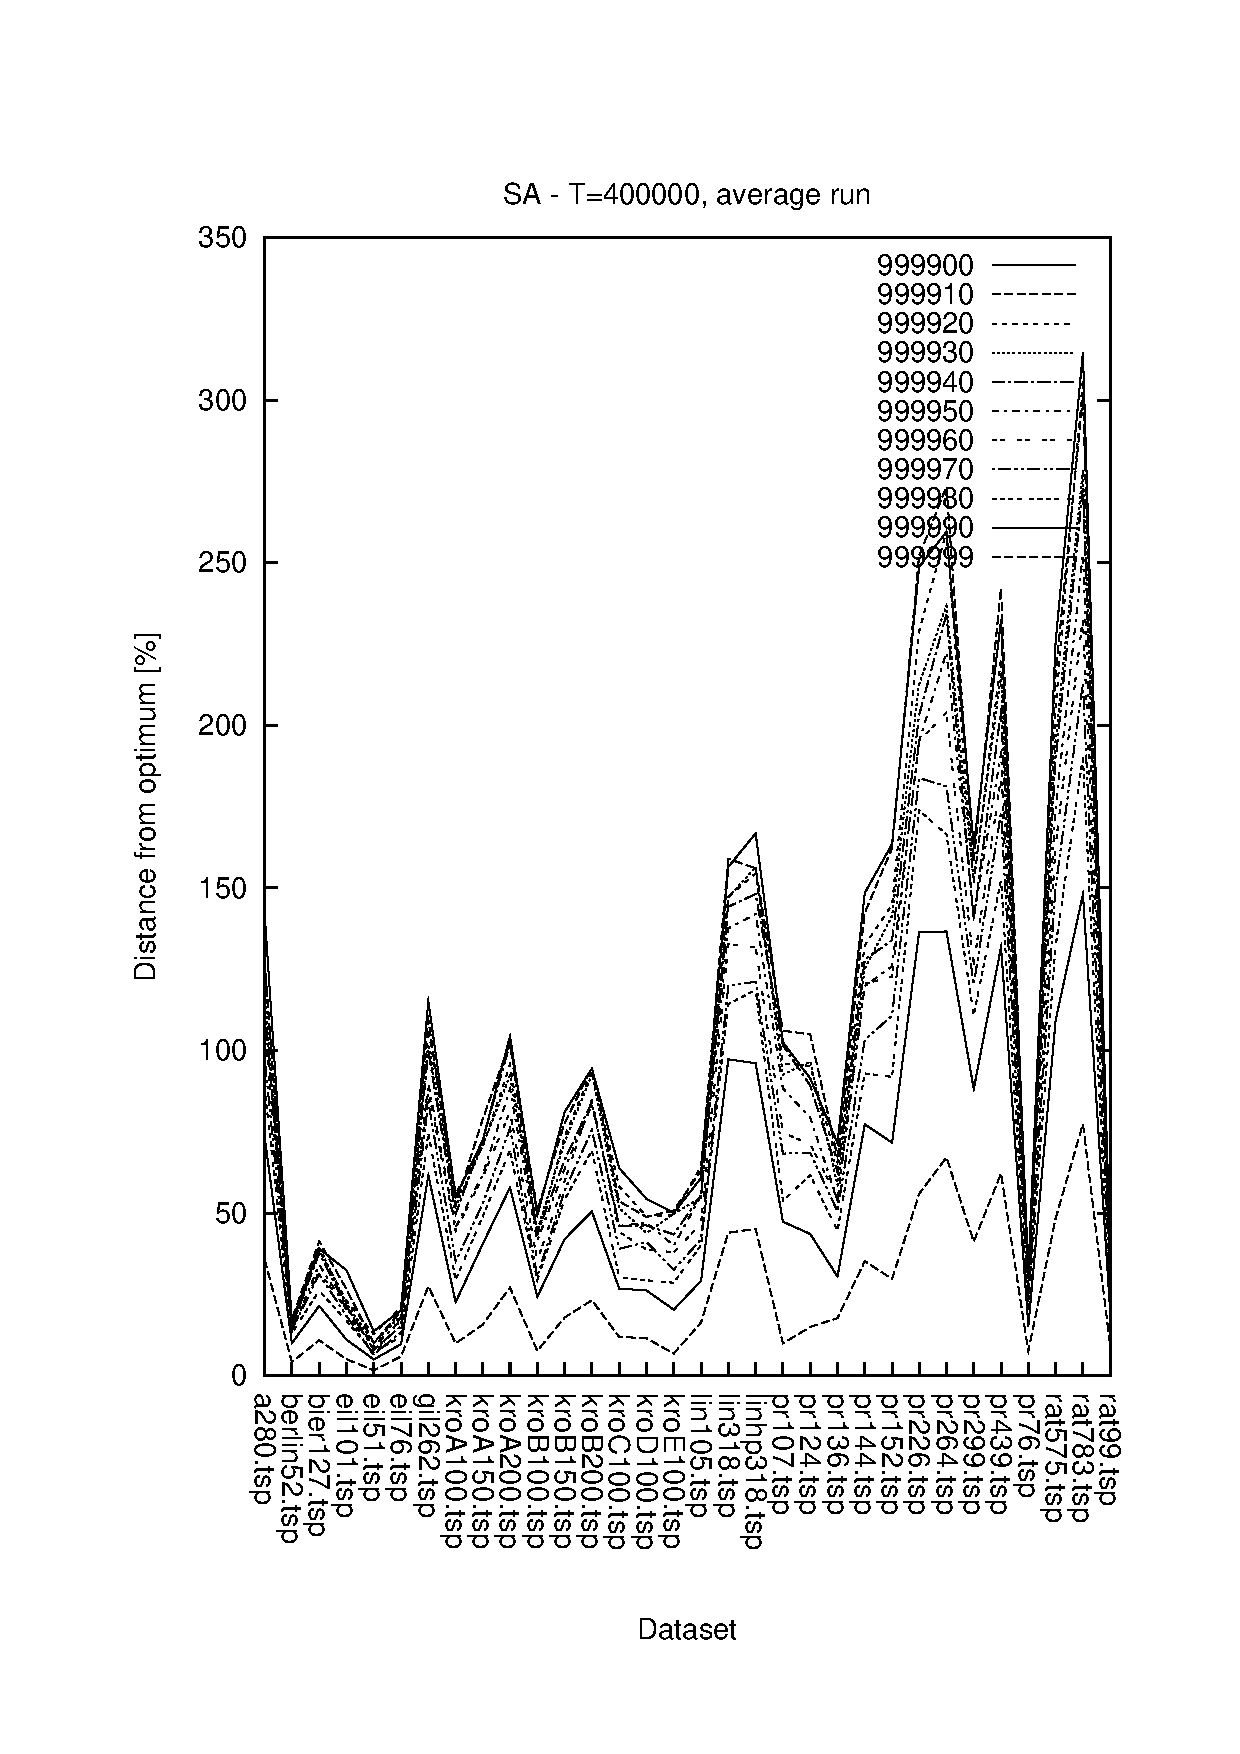
\includegraphics[width=0.9\textwidth]{wykresy/sa/sa_400000_av}
\end{center}
\caption{Porównanie różnych spadków temperatury dla temperatury początkowej 400 000.}
\label{sa_400000_av}
\end{figure}


\begin{figure}
\begin{center}
\includegraphics[width=0.9\textwidth]{wykresy/sa/sa_600000_av}
\end{center}
\caption{Porównanie różnych spadków temperatury dla temperatury początkowej 600 000.}
\label{sa_600000_av}
\end{figure}

\begin{figure}
\begin{center}
\includegraphics[width=0.9\textwidth]{wykresy/sa/sa_1200000_av}
\end{center}
\caption{Porównanie różnych spadków temperatury dla temperatury początkowej 1 200 000.}
\label{sa_1200000_av}
\end{figure}


\begin{figure}
\begin{center}
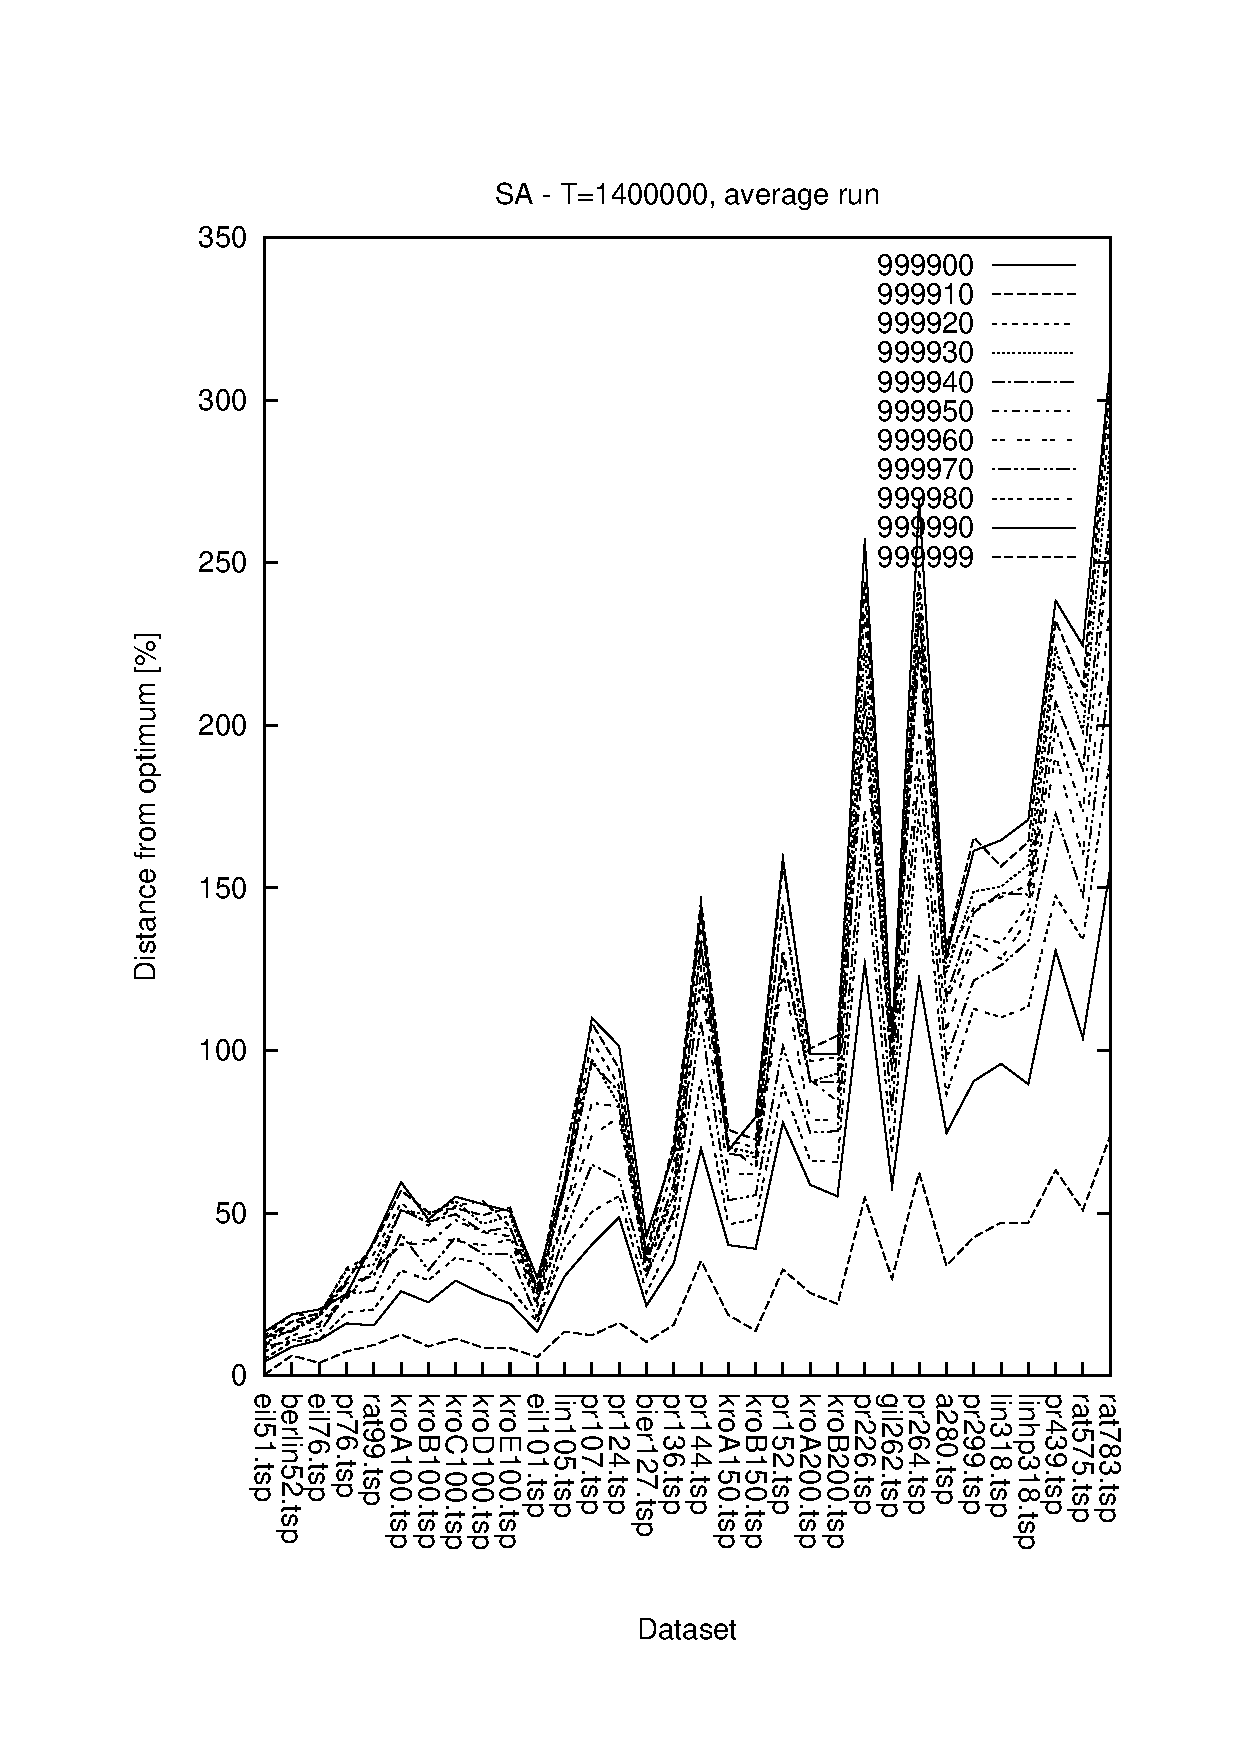
\includegraphics[width=0.9\textwidth]{wykresy/sa/sa_1400000_av}
\end{center}
\caption{Porównanie różnych spadków temperatury dla temperatury początkowej 1 400 000.}
\label{sa_1400000_av}
\end{figure}

\begin{figure}
\begin{center}
\includegraphics[width=0.9\textwidth]{wykresy/sa/sa_1600000_av}
\end{center}
\caption{Porównanie różnych spadków temperatury dla temperatury początkowej 1 600 000.}
\label{sa_1600000_av}
\end{figure}

\begin{figure}
\begin{center}
\includegraphics[width=0.9\textwidth]{wykresy/sa/sa_1800000_av}
\end{center}
\caption{Porównanie różnych spadków temperatury dla temperatury początkowej 1 800 000.}
\label{sa_1800000_av}
\end{figure}

\begin{figure}
\begin{center}
\includegraphics[width=0.9\textwidth]{wykresy/sa/sa_2000000_av}
\end{center}
\caption{Porównanie różnych spadków temperatury dla temperatury początkowej 2 000 000.}
\label{sa_2000000_av}
\end{figure}
